\subsection{RQ1. Comparative Study on C\# Dataset}
\label{rq1:sec}

\begin{table}[t]
	\caption{RQ1. Comparison Results on C\# Dataset for $Accuracy^c$}
	\vspace{-0.1in}
	\begin{center}
		\scriptsize
		\tabcolsep 4pt
		\renewcommand{\arraystretch}{1} \begin{tabular}{p{0.2cm}<{\centering}|p{0.25cm}<{\centering}p{0.25cm}<{\centering}p{0.25cm}<{\centering}|p{0.25cm}<{\centering}p{0.25cm}<{\centering}p{0.25cm}<{\centering}|p{0.25cm}<{\centering}p{0.25cm}<{\centering}p{0.25cm}<{\centering}|p{0.25cm}<{\centering}p{0.25cm}<{\centering}p{0.25cm}<{\centering}|p{0.25cm}<{\centering}p{0.25cm}<{\centering}p{0.25cm}<{\centering}}
			
			\hline
		\multirow{2}{*}{}          & \multicolumn{3}{c|}{Barnett {\em et al.}} & \multicolumn{3}{c|}{Herzig {\em et al.}} & \multicolumn{3}{c|}{$\delta-$PDG + CV} & \multicolumn{3}{c|}{Flexeme} & \multicolumn{3}{c}{\tool}\\
		\cline{2-16}
		 & 2 & 3 & OA & 2 & 3 & OA & 2 & 3 & OA & 2 & 3 & OA & 2 & 3 & OA \\
			\hline
			CL   & 0.14 & *    & 0.14 & 0.28 & *    & 0.28 & 0.34 & *    & 0.34 & 0.34 & *    & 0.34 & 0.46 & *    & 0.46 \\
			CM   & *    & *    & *    & *    & *    & *    & *    & *    & *    & *    & *    & *    & *    & *    & *    \\
			HF   & 0.10 & 0.13 & 0.11 & 0.27 & 0.29 & 0.28 & 0.34 & 0.37 & 0.35 & 0.30 & 0.35 & 0.31 & 0.43 & 0.48 & 0.45 \\
			HU   & 0.13 & *    & 0.13 & 0.27 & *    & 0.27 & 0.30 & *    & 0.30 & 0.33 & *    & 0.33 & 0.44 & *    & 0.44 \\
			LE   & 0.08 & 0.06 & 0.08 & 0.29 & 0.24 & 0.29 & 0.35 & 0.34 & 0.35 & 0.33 & 0.36 & 0.33 & 0.44 & 0.47 & 0.45\\
			NA   & *    & *    & *    & *    & *    & *    & *    & *    & *    & *    & *    & *    & *    & *    & *    \\
			NJ   & 0.07 & *    & 0.07 & 0.28 & *    & 0.28 & 0.34 & *    & 0.34 & 0.27 & *    & 0.27 & 0.41 & *    & 0.41 \\
			NI   & 0.10 & *    & 0.10 & 0.26 & *    & 0.26 & 0.37 & *    & 0.37 & 0.32 & *    & 0.32 & 0.46 & *    & 0.46 \\
			RS   & 0.09 & 0.11 & 0.09 & 0.31 & 0.30 & 0.31 & 0.30 & 0.36 & 0.31 & 0.32 & 0.35 & 0.33 & 0.42 & 0.49 & 0.43\\
			\hline
			OA   & 0.08 & 0.06 & 0.08 & 0.31 & 0.25 & 0.29 & 0.35 & 0.34 & 0.35 & 0.32 & 0.36 & 0.33 & 0.44 & 0.47 & 0.45 \\
			\hline
		\end{tabular}
		\label{RQ1-result-1}
		CM: Commandline, CM: CommonMark, HF:Hangfire, HU: Humanizer, LE: Lean, NA: Nancy, NJ: Newtonsoft.Json, NI: Ninject, RS: RestSharp, OA: Overall, *: No available data point.
	\end{center}
\end{table}

\begin{table}[t]
	\caption{RQ1. Comparison Results on C\# Dataset for $Accuracy^a$}
	\vspace{-0.1in}
	\begin{center}
		\scriptsize
		\tabcolsep 4pt
		\renewcommand{\arraystretch}{1} \begin{tabular}{p{0.2cm}<{\centering}|p{0.25cm}<{\centering}p{0.25cm}<{\centering}p{0.25cm}<{\centering}|p{0.25cm}<{\centering}p{0.25cm}<{\centering}p{0.25cm}<{\centering}|p{0.25cm}<{\centering}p{0.25cm}<{\centering}p{0.25cm}<{\centering}|p{0.25cm}<{\centering}p{0.25cm}<{\centering}p{0.25cm}<{\centering}|p{0.25cm}<{\centering}p{0.25cm}<{\centering}p{0.25cm}<{\centering}}
			
			\hline
			\multirow{2}{*}{}          & \multicolumn{3}{c|}{Barnett {\em et al.}} & \multicolumn{3}{c|}{Herzig {\em et al.}} & \multicolumn{3}{c|}{$\delta-$PDG + CV} & \multicolumn{3}{c|}{Flexeme} & \multicolumn{3}{c}{\tool}\\
			\cline{2-16}
			& 2 & 3 & OA & 2 & 3 & OA & 2 & 3 & OA & 2 & 3 & OA & 2 & 3 & OA \\
			\hline
			CL   & 0.13 & *    & 0.13 & 0.68 & *    & 0.68 & 0.80 & *    & 0.80 & 0.85 & *    & 0.85 & 0.90 & *    & 0.90 \\
			CM   & *    & *    & *    & *    & *    & *    & *    & *    & *    & *    & *    & *    & *    & *    & *    \\
			HF   & 0.06 & 0.11 & 0.07 & 0.71 & 0.59 & 0.68 & 0.81 & 0.86 & 0.82 & 0.80 & 0.89 & 0.82 & 0.84 & 0.91 & 0.86 \\
			HU   & 0.14 & *    & 0.14 & 0.66 & *    & 0.66 & 0.79 & *    & 0.79 & 0.83 & *    & 0.83 & 0.89 & *    & 0.89 \\
			LE   & 0.13 & 0.10 & 0.12 & 0.72 & 0.64 & 0.70 & 0.80 & 0.83 & 0.81 & 0.84 & 0.86 & 0.84 & 0.87 & 0.90 & 0.88\\
			NA   & *    & *    & *    & *    & *    & *    & *    & *    & *    & *    & *    & *    & *    & *    & *    \\
			NJ   & 0.10 & *    & 0.10 & 0.68 & *    & 0.68 & 0.85 & *    & 0.85 & 0.75 & *    & 0.75 & 0.83 & *    & 0.83 \\
			NI   & 0.15 & *    & 0.15 & 0.64 & *    & 0.64 & 0.83 & *    & 0.83 & 0.81 & *    & 0.81 & 0.91 & *    & 0.91 \\
			RS   & 0.12 & 0.17 & 0.13 & 0.76 & 0.78 & 0.76 & 0.74 & 0.81 & 0.76 & 0.82 & 0.87 & 0.83 & 0.87 & 0.88 & 0.87\\
			\hline
			OA   & 0.13 & 0.10 & 0.12 & 0.72 & 0.64 & 0.70 & 0.79 & 0.83 & 0.81 & 0.82 & 0.86 & 0.83 & 0.88 & 0.91 & 0.89 \\
			\hline
		\end{tabular}
		\label{RQ1-result-2}
		CM: Commandline, CM: CommonMark, HF:Hangfire, HU: Humanizer, LE: Lean, NA: Nancy, NJ: Newtonsoft.Json, NI: Ninject, RS: RestSharp, OA: Overall, *: No available data point.
	\end{center}
\end{table}


\textcolor{red}{Yi: consider adding Table 2 in Flexeme paper to our paper on the statistics of the data}.

\textcolor{red}{Yi: add Figure 4(a) in Flexeme paper to our paper to show
  the accuracy distribution for different numbers of concerns.}

Table~\ref{RQ1-result-1} and Table~\ref{RQ1-result-2} show the results about comparing \tool with baselines on C\# dataset. Table~\ref{RQ1-result-1} shows the $Accuracy^c$ results that \tool can improve the $Accuracy^c$ by $462.5\%, 55.2\%, 28.6\%, $ and $36.4\%$ compared with Barnett et al., Herzig et al., $\sigma-$PDG + CV, and Flexeme, respectively. Table~\ref{RQ1-result-2} shows the $Accuracy^a$ results that \tool can improve the  $Accuracy^a$ by $641.7\%, 27.1\%, 9.9\%, $ and $7.3\%$ comparing with Barnett et al., Herzig et al., $\sigma-$PDG + CV, and Flexeme, respectively. On all projects, \tool have the best overall performance compared with baselines, which proves the high accuracy of \tool on untangling task on C\# dataset.


\begin{figure}
	\centering
	\begin{subfigure}{0.2\textwidth}
		\centering
		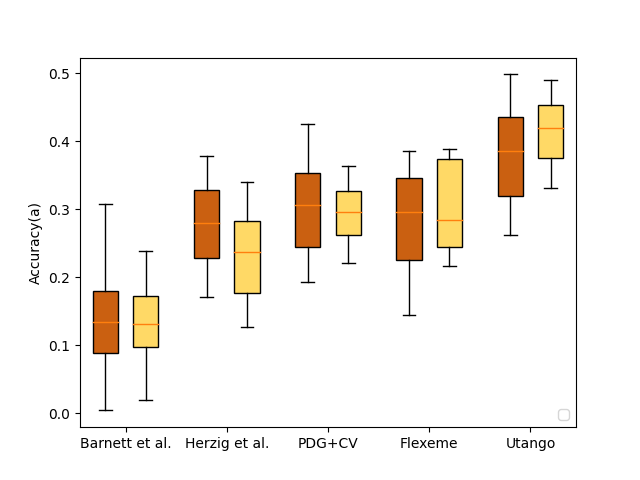
\includegraphics[width=1.4in]{figures/RQ_1_1.png}
		\caption{$Accuracy^c$}
		\label{RQ1-result-3-1}
	\end{subfigure}
	\begin{subfigure}{0.2\textwidth}
		\centering
		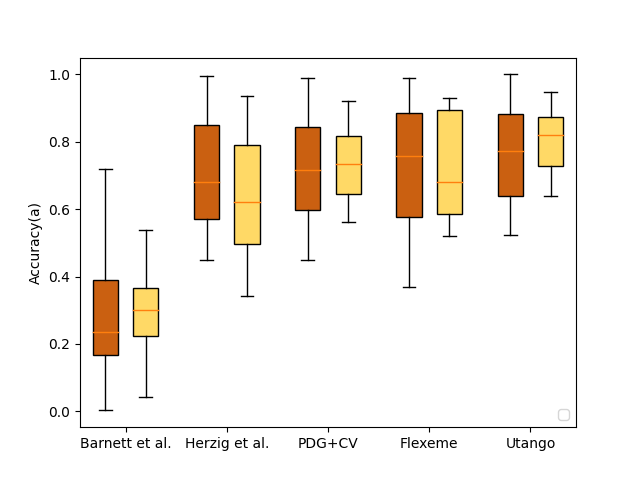
\includegraphics[width=1.4in]{figures/RQ_1_2.png}
		\caption{$Accuracy^a$}
		\label{RQ1-result-3-2}
	\end{subfigure}
	\caption{Boxplots for the Results in Table~\ref{RQ1-result-1} and Table~\ref{RQ1-result-2}. Orange Boxes: 2 concerns data, Yellow Boxes: 3 concerns data}
	\label{RQ1-result-3}
\end{figure}

Figure~\ref{RQ1-result-3} shows the boxplots for both the $Accuracy^c$ and $Accuracy^a$ results in Table~\ref{RQ1-result-1} and Table~\ref{RQ1-result-2}. The orange boxes are for the commits with two concerns, while the yellow boxes are for the commits with three concerns. The results show that the median of the \tool is higher than all baselines on both the two concerns data and three concerns data. By considering the average accuracy reported in Table~\ref{RQ1-result-1} and Table~\ref{RQ1-result-2}, \tool has been proved to have the best results on the C\# dataset when compared with all baselines.

To better understand the performance of \tool, we do an extra analysis on the number of tangled commits that \tool or the best-performed baseline $Flexeme$ can $100\%$ cluster each changed statement correctly. The results show that there are $92$ commits that \tool can $100\%$ cluster the changed statements correctly while there are $64$ commits that $Flexeme$ can $100\%$ cluster the changed statements correctly. The overlapping between them is about $13$ commits. And the concerns in these commits often have $2-9$ statements inside. The number of commits that \tool can $100\%$ correctly cluster changed statements is limited because there are many concerns in the commits containing many changed statements. It is very hard for \tool to cluster each of them correctly at the same time perfectly. That's also why the concerns in $100\%$ correctly clustered commits often have the limited size from $1$ statements to $9$ statements. 

To better understand the performance of \tool on different sizes of concerns, we collect all concerns, and their size is from $1$ statements to $189$ statements. Then, by dividing them into four groups with the same amount of concerns following the order of the size, \tool can achieve $0.49$, $0.47$, $0.44$, and $0.40$ $Accuracy^c$ on group 1 (with the smallest size of concerns) to group 4 (with the biggest size of concerns), respectively. The results show that \tool can perform slightly better on the smaller size of concerns, but the gap on the results is not too big and still in the acceptable range.